\documentclass[border=5mm]{standalone}
\usepackage{luamplib}
\usepackage{graphicx}
\mplibtextextlabel{enable}
\begin{document}
\begin{mplibcode}


beginfig(1);

    picture A;
    A = TEX("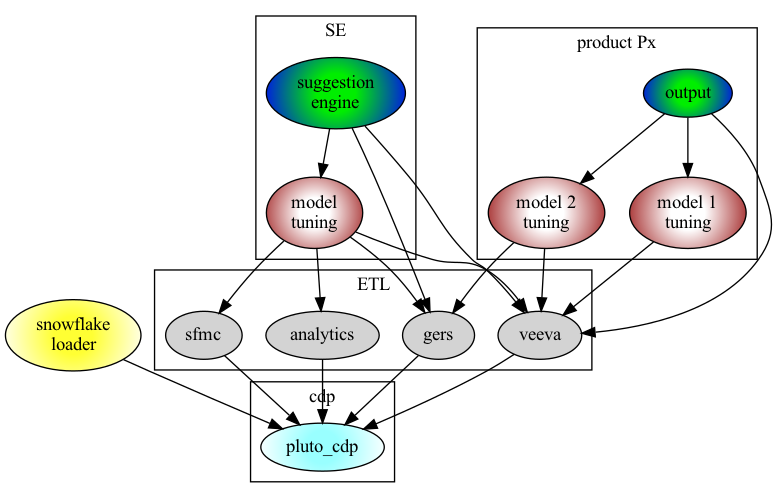
\includegraphics[width=200pt]{archi.png}");

    % alternative, if you like btex ... etex
    % A = btex \includegraphics[width=200pt]{example-image-a} etex;

    draw A scaled .5 ;

    % add a grid (to help you measure the coordinates)
    numeric wd, ht;
    (wd, ht) = urcorner A;
    for x=0 step 10 until wd:
        draw (x, -6) -- (x, ht + 6)
            withcolor if x mod 100 = 0: red else: 7/8 fi;
    endfor
    for y=0 step 10 until ht:
        draw (-6, y) -- (wd + 6, y)
            withcolor if y mod 100 = 0: red else: 7/8 fi;
    endfor

    % add a label (or whatever)
    dotlabel.urt("Label here", (125, 133));
endfig;

\end{mplibcode}
\end{document}
